
\section{Teaching in a Digital Age}

\begin{frame}
  \centering
  From heavy note taking sessions\dots \\
  \begin{minipage}{0.55\linewidth}
    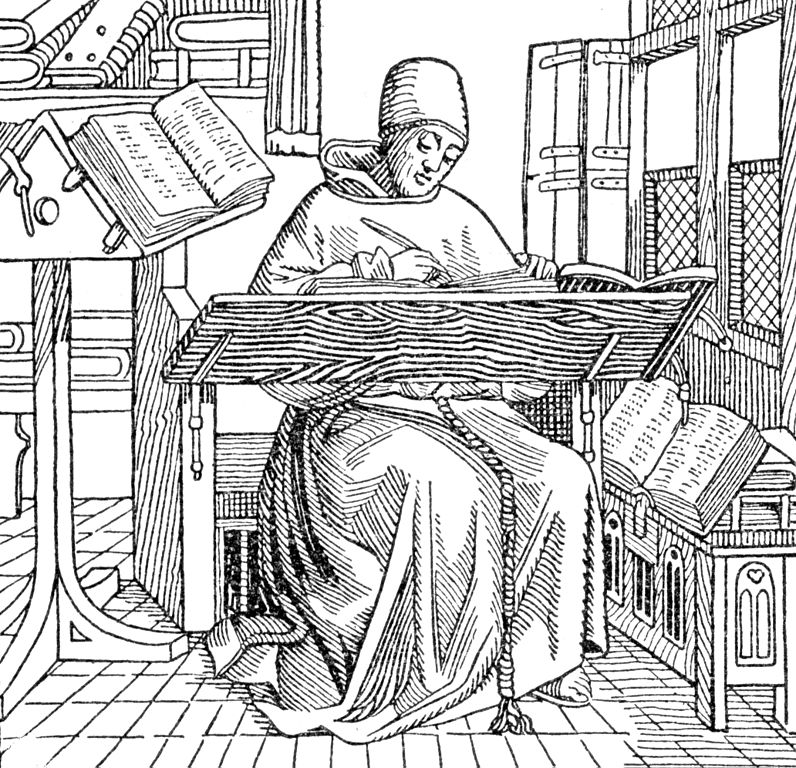
\includegraphics[width=\linewidth,keepaspectratio]{796px-Monkcopyistwoodcut} \\
    \tiny \href{https://commons.wikimedia.org/wiki/File:Monkcopyistwoodcut.jpg}{Wikimedia Commons}
  \end{minipage}
\end{frame}

\begin{frame}
  \centering
  \dots\ to PowerPoint Syndrome \\
  \begin{minipage}{\linewidth}
    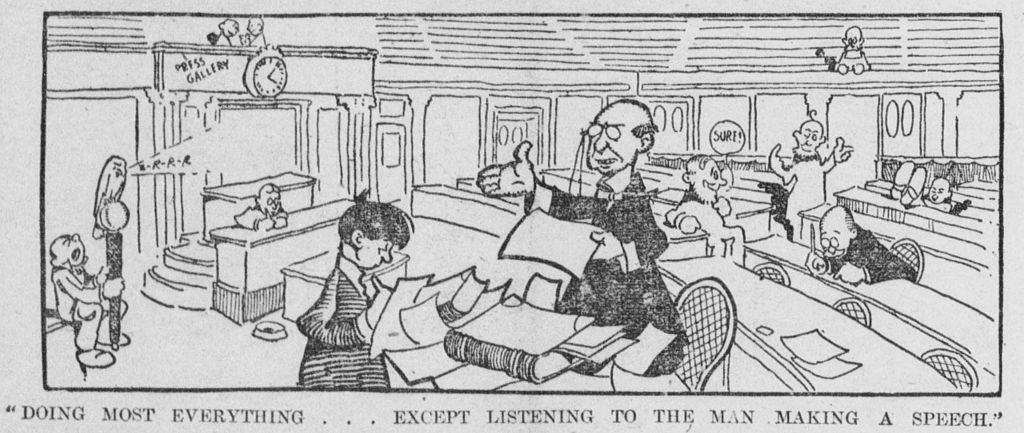
\includegraphics[width=\linewidth,keepaspectratio]{Satterfield_watches_Congress_be_boring} \\
    \tiny \href{https://commons.wikimedia.org/wiki/File:Satterfield_watches_Congress_be_boring.jpg}{Wikimedia Commons}
  \end{minipage}
\end{frame}

\begin{frame}
  \begin{center}
    \textbf{Late 2000s}
  \end{center}
  \begin{center}
    The classroom is obsolete! \\
    \emph{e-learning} is the future!
  \end{center}
\end{frame}

\begin{frame}
  \begin{center}
    \textbf{Pendulum is swinging back}
  \end{center}
  \begin{center}
    Students like to meet their teacher \\
    \pause
    \dots\ provided it's worth it.
  \end{center}
\end{frame}

\begin{frame}[standout]
  Disclaimer \\
  \bigskip

  I am not a specialist.

  Just an ordinary professor\dots \\
  with some experience
\end{frame}

\section{Blended Learning: Identification and Taxonomy}

\begin{frame}
  \frametitle{Definition (One of Many)}

  \begin{quote}
    Thoughtful fusion of face-to-face and online learning experiences
    [\dots] optimally integrated such that \alert{the strengths of
      each} are blended into a unique learning experience congruent
    with the context and intended educational purpose.
    \citep{Garrison:blended:2007}
  \end{quote}
\end{frame}

\begin{frame}
  \frametitle{Models of Blended Learning}

  \begin{description}[Enriched-virtual model]
  \item[Rotation model] Online engagement embedded within face-to-face
    forms of instruction in a cyclical manner
  \item[Flex model] Multiple students engaged primarily online, but
    under the supervision of a teacher who is physically present
  \item[Self-blending model] Students choose different courses to take
    independently, but do so in a setting where a supervising teacher
    and other students are co-present
  \item[\alert<2>{Enriched-virtual model}] Online, virtual experiences are seen
    as being enriched only periodically through arrangements of
    physical co-presence
  \end{description}

  \citep{Stalker:blended:2012,Friesen:blended:2012}

\end{frame}

\begin{frame}
  \frametitle{Continuum of Technology-Based Learning}

  \centering
  \begin{minipage}{0.75\linewidth}
    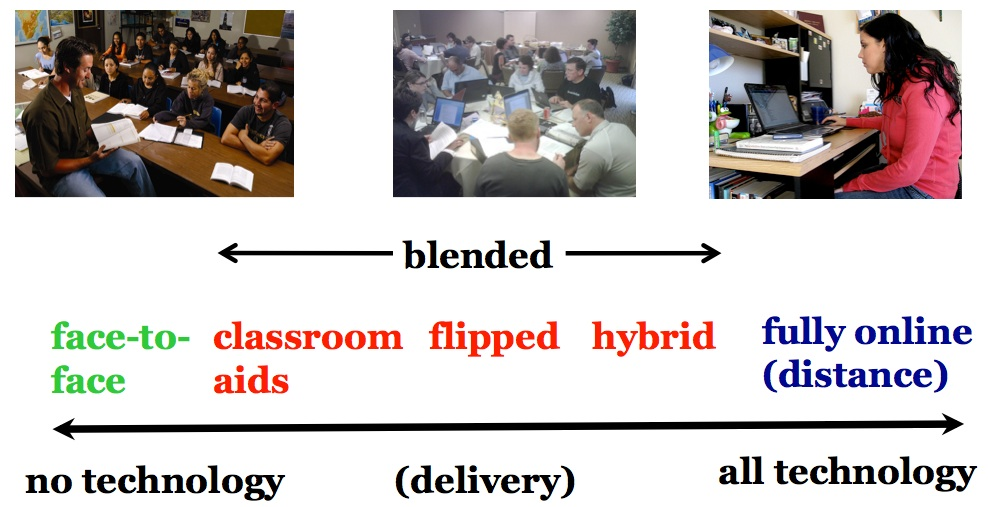
\includegraphics[width=\linewidth,keepaspectratio]{Continuum-of-technology-based-teaching-2} \\
    \tiny \citet{Bates:digital:2015}
  \end{minipage}
  \vfill
  \mbox{}

  \only<2->{
    \begin{textblock*}{40mm}[1,0](85mm,80mm)
      \small\raggedleft%
      lectures prepared online before meeting in class
    \end{textblock*}
    \begin{textblock*}{0mm}(80mm,78mm)
      \setlength{\unitlength}{1mm}
      \begin{picture}(0,0)
        \color{alert}
        \put(-8,21){\framebox(16,6.5)[bl]{}}
        \put(0,0){\line(0,1){21}}
      \end{picture}
    \end{textblock*}}

  \only<3->{
    \begin{textblock*}{60mm}(92mm,80mm)
      \small\raggedright%
      majority of learning online, class only for very specific
      face-to-face teaching that cannot be done satisfactorily online
    \end{textblock*}
    \begin{textblock*}{0mm}(97mm,78mm)
      \setlength{\unitlength}{1mm}
      \begin{picture}(0,0)
        \color{alert}
        \put(-8,21){\framebox(16,6.5)[bl]{}}
        \put(0,0){\line(0,1){21}}
      \end{picture}
    \end{textblock*}}
\end{frame}


\section{How I Stopped Worrying \newline and Love Blended Learning}

\begin{frame}[fragile=singleslide]
  \frametitle{Context}

  \begin{itemize}
  \item Numerical Methods course with R Programming component
  \item Teaching of programming part further \alert{left} on the blended
    learning continuum
    \begin{center}
      \medskip
      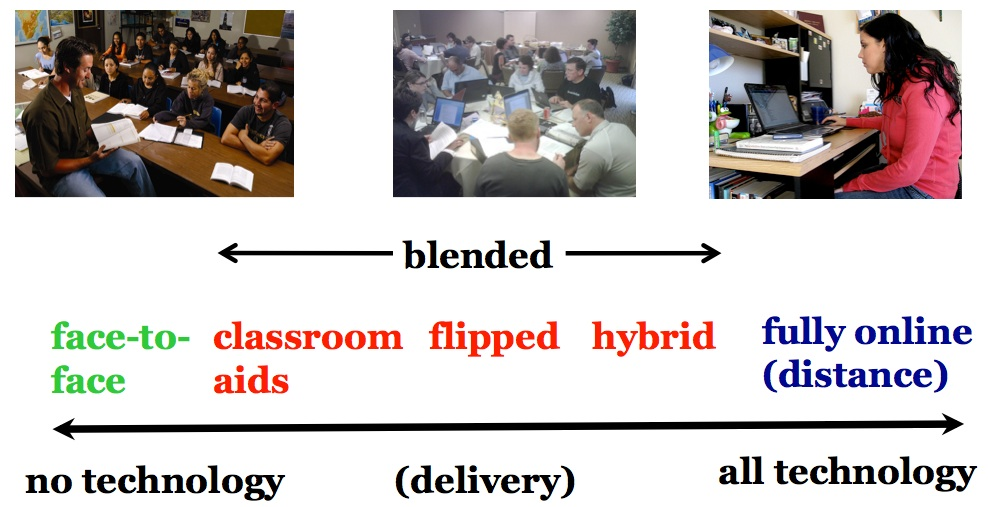
\includegraphics[width=0.7\linewidth,keepaspectratio,%
        trim=0 0 0 230,clip]{Continuum-of-technology-based-teaching-2}
      \setlength{\unitlength}{1mm}
      \begin{picture}(0,0)
        \color{alert}
        \put(-75,10){\framebox(19.8,8)[bl]{}}
      \end{picture}
    % \begin{minipage}{0.3\linewidth}
    %   \includegraphics[width=\linewidth,keepaspectratio,frame]{slides-extract.png} \\
    %   \includegraphics[width=\linewidth,keepaspectratio,frame]{bases-extract.png} \\
    % \end{minipage}
    \end{center}

  \item Strong push towards fully online (distance) learning at Université Laval
  \end{itemize}
\end{frame}

\begin{frame}
  \frametitle{Motivation}

  \begin{itemize}
  \item \alert{Not} to increase course accessibility
  \item Administrative duties
    \begin{itemize}
    \item looking for a more free-standing course
    \end{itemize}
  \item Ineffectiveness of assignments
    \begin{itemize}
    \item no feedback to students
    \item complaints about workload
    \end{itemize}
  \end{itemize}
\end{frame}

%% These are defined outside the following frame to avoid troubles
%% with overlays.
\setlength{\unitlength}{1mm}
\newsavebox{\activity}
\savebox{\activity}(4,0){\color{alert}\circle*{4}}
\newsavebox{\week}
\savebox{\week}(12,0){\color{dark}\rule[-1mm]{12mm}{2mm}}

\begin{frame}
  \frametitle{My Hybrid Teaching Model}
  \centering
  \begin{picture}(125,60)
    \put(0,40){\usebox{\activity}}
    \put(4,40){\usebox{\week}}
    \put(18,40){\usebox{\week}} \put(30,40){\usebox{\activity}}
    \put(34,40){\usebox{\week}} \put(46,40){\usebox{\activity}}
    \put(50,40){\usebox{\week}}
    \put(64,40){\usebox{\week}} \put(70,44){\makebox(0,0){\color{alert}\faPlusSquare}}
    \put(78,40){\usebox{\week}} \put(90,40){\usebox{\activity}}
    \put(94,40){\usebox{\week}}
    \multiput(109,40)(2.5,0){3}{\circle*{0.7}}

    \only<2->{
      \put(0,37.5){\line(0,-1){31}}
      \put(1,30){%
        \begin{minipage}[t]{35mm}
          \faUsers \\ Launch activity
          \begin{itemize}
          \item welcome
          \item course outline
          \item software install
          \end{itemize}
        \end{minipage}}
    }

    \only<3->{
      \put(40,37.5){\line(0,-1){31}}
      \put(41,30){%
        \begin{minipage}[t]{50mm}
          \faUser \\ Independent work
          \begin{itemize}
          \item theory and examples
          \item exercices
          \item formative assessments
          \end{itemize}
        \end{minipage}}
    }

    \only<4->{
      \put(90,37.5){\line(0,-1){26}}
      \put(91,30){%
        \begin{minipage}[t]{35mm}
          \faUsers \\ Classroom activities
          \begin{itemize}
          \item review of material
          \item team project
          \end{itemize}
        \end{minipage}}
    }

    \only<5->{
      \put(70,46.2){\line(0,1){12}}
      \put(71,50){%
        \parbox[b]{30mm}{\faShareAlt \\ Online tutorial}}
    }
  \end{picture}
\end{frame}

\section{Demo}

\section{Field Report}

\begin{frame}
  \frametitle{Students Feedback}

  \begin{minipage}{0.48\textwidth}
    They like
    \begin{itemize}
    \item Autonomy
    \item Flexible schedule
    \item Variety of learning experiences
    \end{itemize}
  \end{minipage}
  \hfill
  \begin{minipage}{0.48\textwidth}
    They like less
    \begin{itemize}
    \item Autonomy
    \item Apparent lack of supervision
    \item Time constrained (60~min.) projects
    \end{itemize}
  \end{minipage}
\end{frame}

\begin{frame}
  \frametitle{Tips and Tricks}

  \begin{itemize}[<+->]
  \item Trust the students
  \item Don't trust the students ;-)
  \end{itemize}

  \begin{itemize}[<3->]
  \item Plan, starting from learning objectives
  \item Provide a clear roadmap
  \item Vary learning experiences
  \item Write exam questions congruent with learning objectives
  \item Avoid overengineering
  \end{itemize}

  \begin{itemize}[<4->]
  \item You will need a learning management system (LMS)
  \end{itemize}
\end{frame}

%%% Local Variables:
%%% mode: latex
%%% TeX-engine: xetex
%%% TeX-master: "atc-2017-blended-learning"
%%% End:
